%beamer

% Define a global usable date. Must come before StyleTut
% \newcommand{\mydate}{04.11.2016}

% Comment/uncomment this line to toggle handout mode
% \newcommand{\handout}{}

%% Beamer-Klasse im korrekten Modus
\ifdefined \handout
\documentclass[handout]{beamer} % Handout mode
\else
\documentclass{beamer}
\fi

%% UTF-8-Encoding
\usepackage[utf8]{inputenc}

% % \bigtimes abgeschrieben von http://tex.stackexchange.com/questions/14386/importing-a-single-symbol-from-a-different-font
% \DeclareFontFamily{U}{mathx}{\hyphenchar\font45}
% \DeclareFontShape{U}{mathx}{m}{n}{
%       <5> <6> <7> <8> <9> <10> gen * mathx
%       <10.95> mathx10 <12> <14.4> <17.28> <20.74> <24.88> mathx12
%       }{}
% \DeclareSymbolFont{mathx}{U}{mathx}{m}{n}
% \DeclareMathSymbol{\bigtimes}{\mathop}{mathx}{161}

\RequirePackage{xcolor}

\def\9{\square}
%\def\9{\blank}

% f"ur Aussagenlogik
\colorlet{alcolor}{blue}
\RequirePackage{tikz}
\usetikzlibrary{arrows.meta}
\newcommand{\alimpl}{\mathrel{\tikz[x={(0.1ex,0ex)},y={(0ex,0.1ex)},>={Classical TikZ Rightarrow[]}]{\draw[alcolor,->,line width=0.7pt,line cap=round] (0,0) -- (15,0);\path (0,-6);}}}
\newcommand{\aleqv}{\mathrel{\tikz[x={(0.1ex,0ex)},y={(0ex,0.1ex)},>={Classical TikZ Rightarrow[]}]{\draw[alcolor,<->,line width=0.7pt,line cap=round] (0,0) -- (18,0);\path (0,-6);}}}
\newcommand{\aland}{\mathbin{\raisebox{-0.6pt}{\rotatebox{90}{\texttt{\color{alcolor}\char62}}}}}
\newcommand{\alor}{\mathbin{\raisebox{-0.8pt}{\rotatebox{90}{\texttt{\color{alcolor}\char60}}}}}
%\newcommand{\ali}[1]{_{\mathtt{\color{alcolor}#1}}}
\newcommand{\alv}[1]{\mathtt{\color{alcolor}#1}}
\newcommand{\alnot}{\mathop{\tikz[x={(0.1ex,0ex)},y={(0ex,0.1ex)}]{\draw[alcolor,line width=0.7pt,line cap=round,line join=round] (0,0) -- (10,0) -- (10,-4);\path (0,-8) ;}}}
\newcommand{\alP}{\alv{P}} %ali{#1}}
%\newcommand{\alka}{\negthinspace\hbox{\texttt{\color{alcolor}(}}}
\newcommand{\alka}{\negthinspace\text{\texttt{\color{alcolor}(}}}
%\newcommand{\alkz}{\texttt{\color{alcolor})}}\negthinspace}
\newcommand{\alkz}{\text{\texttt{\color{alcolor})}}\negthinspace}
\newcommand{\AAL}{A_{AL}}
\newcommand{\LAL}{\hbox{\textit{For}}_{AL}}
\newcommand{\AxAL}{\hbox{\textit{Ax}}_{AL}}
\newcommand{\AxEq}{\hbox{\textit{Ax}}_{Eq}}
\newcommand{\AxPL}{\hbox{\textit{Ax}}_{PL}}
\newcommand{\AALV}{\hbox{\textit{Var}}_{AL}}
\newcommand{\MP}{\hbox{\textit{MP}}}
\newcommand{\GEN}{\hbox{\textit{GEN}}}
\newcommand{\W}{\ensuremath{\hbox{\textbf{w}}}\xspace}
\newcommand{\F}{\ensuremath{\hbox{\textbf{f}}}\xspace}
\newcommand{\WF}{\ensuremath{\{\W,\F\}}\xspace}
\newcommand{\val}{\hbox{\textit{val}}}
\newcommand{\valDIb}{\val_{D,I,\beta}}

\newcommand*{\from}{\colon}

% die nachfolgenden Sachen angepasst an cmtt
\newlength{\ttquantwd}
\setlength{\ttquantwd}{1ex}
\newlength{\ttquantht}
\setlength{\ttquantht}{6.75pt}
\def\plall{%
  \tikz[line width=0.67pt,line cap=round,line join=round,baseline=(B),alcolor] {
    \draw (-0.5\ttquantwd,\ttquantht) -- node[coordinate,pos=0.4] (lll){} (-0.25pt,-0.0pt) -- (0.25pt,-0.0pt) -- node[coordinate,pos=0.6] (rrr){} (0.5\ttquantwd,\ttquantht);
    \draw (lll) -- (rrr);
    \coordinate (B) at (0,-0.35pt);
  }%
}
\def\plexist{%
  \tikz[line width=0.67pt,line cap=round,line join=round,baseline=(B),alcolor] {
    \draw (-0.9\ttquantwd,\ttquantht) -- (0,\ttquantht) -- node[coordinate,pos=0.5] (mmm){} (0,0) --  (-0.9\ttquantwd,0);
    \draw (mmm) -- ++(-0.75\ttquantwd,0);
    \coordinate (B) at (0,-0.35pt);
  }\ensuremath{\,}%
}
\let\plexists=\plexist
\newcommand{\NT}[1]{\ensuremath{\langle\mathrm{#1} \rangle}}

\newcommand{\CPL}{\text{\itshape Const}_{PL}}
\newcommand{\FPL}{\text{\itshape Fun}_{PL}}
\newcommand{\RPL}{\text{\itshape Rel}_{PL}}
\newcommand{\VPL}{\text{\itshape Var}_{PL}}
\newcommand{\ATer}{A_{\text{\itshape Ter}}}
\newcommand{\ARel}{A_{\text{\itshape Rel}}}
\newcommand{\AFor}{A_{\text{\itshape For}}}
\newcommand{\LTer}{L_{\text{\itshape Ter}}}
\newcommand{\LRel}{L_{\text{\itshape Rel}}}
\newcommand{\LFor}{L_{\text{\itshape For}}}
\newcommand{\NTer}{N_{\text{\itshape Ter}}}
\newcommand{\NRel}{N_{\text{\itshape Rel}}}
\newcommand{\NFor}{N_{\text{\itshape For}}}
\newcommand{\PTer}{P_{\text{\itshape Ter}}}
\newcommand{\PRel}{P_{\text{\itshape Rel}}}
\newcommand{\PFor}{P_{\text{\itshape For}}}

\newcommand{\plka}{\alka}
\newcommand{\plkz}{\alkz}
%\newcommand{\plka}{\plfoo{(}}
%\newcommand{\plkz}{\plfoo{)}}
\newcommand{\plcomma}{\hbox{\texttt{\color{alcolor},}}}
\newcommand{\pleq}{{\color{alcolor}\,\dot=\,}}

% MODIFIED (DJ)
% previously: \newcommand{\plfoo}[1]{\mathtt{\color{alcolor}#1}}
\newcommand{\plfoo}[1]{\texttt{\color{alcolor}#1}}

\newcommand{\plc}{\plfoo{c}}
\newcommand{\pld}{\plfoo{d}}
\newcommand{\plf}{\plfoo{f}}
\newcommand{\plg}{\plfoo{g}}
\newcommand{\plh}{\plfoo{h}}
\newcommand{\plx}{\plfoo{x}}
\newcommand{\ply}{\plfoo{y}}
\newcommand{\plz}{\plfoo{z}}
\newcommand{\plR}{\plfoo{R}}
\newcommand{\plS}{\plfoo{S}}

\newcommand{\bv}{\mathrm{bv}}
\newcommand{\fv}{\mathrm{fv}}

%\newcommand{\AxAL}{\hbox{\textit{Ax}}_{AL}}
%\newcommand{\AALV}{\hbox{\textit{Var}}_{AL}}

%\renewcommand{\#}[1]{\literal{#1}}
\newcommand{\A}{\mathcal{A}}
\newcommand{\Adr}{\text{Adr}}
\newcommand{\ar}{\mathrm{ar}}
\newcommand{\ascii}[1]{\literal{\char#1}}
%\newcommand{\assert}[1]{\text{/\!\!/\ } #1}
\newcommand{\assert}[1]{\colorbox{black!7!white}{\ensuremath{\{\;#1\;\}}}}
\newcommand{\Assert}[1]{$\langle$\textit{#1}$\rangle$}
\newcommand{\B}{\mathcal{B}}
\newcommand{\bfmod}{\mathbin{\kw{ mod }}}
\newcommand{\bb}{{\text{bb}}}
\def\bottom{\hbox{\small$\pmb{\bot}$}}
\newcommand{\card}[1]{|#1|}
%\newcommand{\cod}{\mathop{\text{cod}}}  % ist in thwmathabbrevs
\newcommand{\Conf}{\mathcal{C}}
\newcommand{\define}[1]{\emph{#1}}
%\renewcommand{\dh}{d.\,h.\@\xspace}
%\newcommand{\Dh}{D.\,h.\@\xspace}
%\newcommand{\engl}[1]{engl.\xspace\emph{#1}}
\newcommand{\eps}{\varepsilon}
%\newcommand{\evtl}{evtl.\@\xspace}
\newcommand{\fbin}{\text{bin}}
\newcommand{\finv}{\text{inv}}
\newcommand{\fnum}{\text{num}}
\newcommand{\fNum}{{\text{Num}}}
\newcommand{\frepr}{\text{repr}}
\newcommand{\fRepr}{\text{Repr}}
\newcommand{\fZkpl}{\text{Zkpl}}
\newcommand{\fLen}{\text{Len}}
\newcommand{\fsem}{\text{sem}}
\providecommand{\fspace}{\mathord{\text{space}}}
\providecommand{\fSpace}{\mathord{\text{Space}}}
\providecommand{\ftime}{\mathord{\text{time}}}
\providecommand{\fTime}{\mathord{\text{Time}}}
\newcommand{\fTrans}{\text{Trans}}
\newcommand{\fVal}{\text{Val}}

% Modified (DJ)
\newcommand{\Val}{\text{Val}}

%\def\G{\mathbb{Z}}
\newcommand{\HT}[1]{\normalfont\textsc{HT-#1}}
\newcommand{\htr}[3]{\{#1\}\;#2\; \{#3\}}
\newcommand{\Id}{\text{I}}
%\newcommand{\ie}{i.\,e.\@\xspace}
\newcommand{\instr}[2]{\texttt{#1}\ \textit{#2}}
\newcommand{\Instr}[2]{\texttt{#1}\ \textrm{#2}}
\newcommand{\instrr}[3]{\texttt{#1}\ \textit{#2}\texttt{(#3)}}
\newcommand{\Instrr}[3]{\texttt{#1}\ \textrm{#2}\texttt{(#3)}}
\newcommand{\io}{\!\mid\!}
\usepackage{KITcolors}
\newcommand{\literal}[1]{\hbox{\textcolor{blue!95!white}{\textup{\texttt{\scalebox{1.11}{#1}}}}}}
%\newcommand{\literal}[1]{\hbox{\textcolor{KITblue!80!black}{\textup{\texttt{#1}}}}}
\def\kasten#1{\leavevmode\literal{\setlength{\fboxsep}{1pt}\fbox{\vrule  width 0pt height 1.5ex depth 0.5ex #1}}}
\newcommand{\kw}[1]{\ensuremath{\mathbf{#1}}}
\newcommand{\lang}[1]{\ensuremath{\langle#1\rangle}}
%\newcommand{\maw}{m.\,a.\,w.\@\xspace}
%\newcommand{\MaW}{M.\,a.\,w.\@\xspace}
\newcommand{\mdefine}[2][FOOBAR]{\define{#2}\def\foobar{FOOBAR}\def\optarg{#1}\ifx\foobar\optarg\def\optarg{#2}\fi\graffito{\optarg}}
\newcommand{\meins}{\rotatebox[origin=c]{180}{1}}
\newcommand{\Mem}{\text{Mem}}
\newcommand{\memread}{\text{memread}}
\newcommand{\memwrite}{\text{memwrite}}
\providecommand{\meta}[1]{\ensuremath{\langle}\textit{#1}\ensuremath{\rangle}}
%\newcommand{\N}{\mathbb{N}}
\newcommand{\NP}{\mathbf{NP}}
\newcommand{\Nadd}{N_{\text{add}}}
\newcommand{\Nmult}{N_{\text{mult}}}
\newcommand{\Oh}[1]{O\left(#1\right)}
\newcommand{\Om}[1]{\Omega\left(#1\right)}
\newcommand{\personname}[1]{\textsc{#1}}
\newcommand{\regname}[1]{\texttt{#1}}
\newcommand{\mima}{\textsc{Mima}\xspace}
\newcommand{\mimax}{\textsc{Mima-X}\xspace}

\def\Pclass{\text{\bfseries P}}
\def\PSPACE{\text{\bfseries PSPACE}}

\newcommand{\SPush}{\text{push}}
\newcommand{\SPop}{\text{pop}}
\newcommand{\SPeek}{\text{peek}}
\newcommand{\STop}{\text{top}}
\newcommand{\STos}{\text{\itshape tos}}
\newcommand{\SBos}{\text{\itshape bos}}

%\newcommand{\R}{\mathbb{R}}
\newcommand{\Rnullplus}{\R_0^{+}}
\newcommand{\Rplus}{\R_{+}}
\newcommand{\resp}{resp.\@\xspace}
\newcommand{\Sem}{\text{Sem}}
\newcommand{\sgn}{\mathop{\text{sgn}}}
\newcommand{\sqbox}{\mathop{\raisebox{-6.2pt}{\hbox{\hbox to 0pt{$^{^{\sqcap}}$\hss}$^{^{\sqcup}}$}}}}
\newcommand{\sqleq}{\sqsubseteq}
\newcommand{\sqgeq}{\sqsupseteq}
\newcommand{\Th}[1]{\Theta\left(#1\right)}
%\newcommand{\usw}{usw.\@\xspace}
\newcommand{\V}[1]{\hbox{\textit{#1}}}
\newcommand{\x}{\times}
\newcommand{\ZK}{\mathbb{K}}
%\newcommand{\Z}{\mathbb{Z}}
%\newcommand{\zB}{z.\,B.\@\xspace}
%\newcommand{\ZB}{Z.\,B.\@\xspace}
% \newcommand{\bb}{{\text{bb}}}
% \def\##1{\hbox{\textcolor{darkblue}{\texttt{#1}}}}
% \def\A{\mathcal{A}}
% \newcommand{\0}{\#0}
% \newcommand{\1}{\#1}
% \newcommand{\Obj}{\text{Obj}}
% \newcommand{\start}{\mathop{\text{start}}}
% \newcommand{\compactlist}{\addtolength{\itemsep}{-\parskip}}
% \newcommand{\fval}{\text{val}}
% \newcommand{\lang}[1]{\ensuremath{\langle#1\rangle}}
% \newcommand{\io}{\!\mid\!}
% \def\sqbox{\mathop{\raisebox{-6.2pt}{\hbox{\hbox to 0pt{$^{^{\sqcap}}$\hss}$^{^{\sqcup}}$}}}}
% \def\sqleq{\sqsubseteq}
% \def\sqgeq{\sqsupseteq}
\def\Td{T_{\overline{d}}}
% \newcommand{\csym}[1]{\ensuremath{\#{c}_{\#{\hbox{\scriptsize #1}}}}}
% \newcommand{\F}{\ensuremath{\mathcal{F}}}
% \newcommand{\fsym}[2]{\ensuremath{\#{f}^{\#{\hbox{\scriptsize #1}}}_{\#{\hbox{\scriptsize #2}}}}}
% \newcommand{\rsym}[2]{\ensuremath{\#{R}^{\#{\hbox{\scriptsize #1}}}_{\#{\hbox{\scriptsize #2}}}}}
% \newcommand{\xsym}[1]{\ensuremath{\#{x}_{\#{\hbox{\scriptsize #1}}}}}
% \newcommand{\I}{\mathcal{I}}
% ********************************************************************

\usepackage{../TutTexbib/thwregex}
\usepackage{environ}
\usepackage{bm}
\usepackage{calc}
\usepackage{varwidth}
\usepackage{wasysym}
\usepackage{mathtools}

%% Tabellen
\usepackage{array}
\usepackage{multicol}

%% Bibliotheken für viele mathematische Symbole
\usepackage{amsmath, amsfonts, amssymb}



% This is a configuration file with personal tutor information.
% It is therefore excluded from the git repository, so changes in this file will not conflict in git commits.

% Copy this template, rename to config.tex and add your information below.

\newcommand{\myname}{Lukas Morawietz}
\newcommand{\mymail}{lukas.morawietz@gmail.com} % Consider using your named student mail address to keep your u**** account private.
\newcommand{\mytutnumber}{31}

% Don't forget to update ILIAS url. WARNING: Underscores '_' and Ampersands '&' have to be escaped with backslashes '\'. Blame TeX, not me.
\newcommand{\myILIASurl}{https://ilias.studium.kit.edu/ilias.php?ref\_id=855240\&cmdClass=ilrepositorygui\&cmdNode=5r\&baseClass=ilrepositorygui}

% Uncommenting this will print Socrative info with here defined roomname whenever \Socrative is called.
% (Otherwise, \Socrative will remain silent.)
% \newcommand{\mysocrativeroom}{???}

%\def\ThassesTut{}
\def\DanielsTut{}

\newcommand{\aboutMeFrame}{
	\begin{frame}{Über mich}
		\myname \\
		Informatik, 9. Fachsemester (Bachelor)
		% Lebensgeschichte...
		% Stammbaum...
		% Aufarbeitung der eigenen Todesser-Vergangenheit...
	\end{frame}
}

\def\thisyear{2019}

% Update date of exam
\def\myKlausurtermin{18.~März~2020, 14:00–16:00~Uhr}

\def\mydate#1{
		  \ifnum#1=1\relax	  23. Oktober \thisyear \
	\else \ifnum#1=2\relax	  30. Oktober \thisyear \
	\else \ifnum#1=3\relax    06. November \thisyear \
	\else \ifnum#1=4\relax    13. November \thisyear \
	\else \ifnum#1=5\relax    20. November \thisyear \
	\else \ifnum#1=6\relax    27. November \thisyear \
	\else \ifnum#1=7\relax    04. Dezember \thisyear \
	\else \ifnum#1=8\relax    11. Dezember \thisyear \
	\else \ifnum#1=9\relax    18. Dezember \thisyear \
	\else \ifnum#1=10\relax   08. Januar \nextyear \
	\else \ifnum#1=11\relax   15. Januar \nextyear \
	\else \ifnum#1=12\relax   22. Januar \nextyear \
	\else \ifnum#1=13\relax   29. Januar \nextyear \
	\else \ifnum#1=14\relax   05. Februar \nextyear \
	\else \textbf{Datum undefiniert!} 
	\fi\fi\fi\fi\fi\fi\fi\fi\fi\fi\fi\fi\fi\fi
}

\def\mylasttimestext{Was letztes Mal geschah...}

\colorlet{beamerlightred}{red!40}
\colorlet{beamerlightgreen}{green!50}
\colorlet{beamerlightyellow}{yellow!50}
\colorlet{lightred}{red!30}
\colorlet{lightgreen}{green!40}
\colorlet{lightyellow}{yellow!50}
\colorlet{fullred}{red!60}
\colorlet{fullgreen}{green}

\definecolor{myalertcolor}{rgb}{1,0.33,0.24}
\setbeamercolor{alerted text}{fg=myalertcolor}

% Flag to toggle display of KIT Logo.
% If you want to conform to the official logo guidelines, 
% you are not allowed to use the logo and should disable it
% using the following flag. Just saying.
% (But it's too beautiful, so best leave this commented. :P)
%\newcommand{\noKITLogo}{}

% Toggle handout mode by including the following line before including PraeambelTut
% and removing the % at the start (but do NOT remove the % char here, otherwise handout mode will always be on!)
% Please keep handout mode off in all commits!

% \newcommand{\handout}{}



% define custom \handout command flag if handout mode is toggled  #DirtyAsHellButWell...
\only<beamer:0>{\def\handout{}} %beamer:0 == handout mode

\newcommand{\R}{\mathbb{R}}
\newcommand{\N}{\mathbb{N}}
\newcommand{\Z}{\mathbb{Z}}
\newcommand{\Q}{\mathbb{Q}}
\newcommand{\BB}{\mathbb{B}}
\newcommand{\C}{\mathbb{C}}
\newcommand{\K}{\mathbb{K}}
\newcommand{\G}{\mathbb{G}}
\newcommand{\nullel}{\mathcal{O}}
\newcommand{\einsel}{\mathds{1}}
\newcommand{\Pot}{\mathcal{P}}
\renewcommand{\O}{\text{O}}

\def\word#1{\hbox{\textcolor{blue}{\texttt{#1}}}}
\let\literal\word
\def\mword#1{\hbox{\textcolor{blue}{$\mathtt{#1}$}}}  % math word
\def\sp{\scalebox{1}[.5]{\textvisiblespace}}
\def\wordsp{\word{\sp}}

%\newcommand{\literal}[1]{\textcolor{blue}{\texttt{#1}}}
\newcommand{\realTilde}{\textasciitilde \ }
\newcommand{\setsize}[1]{\ensuremath{\left\lvert #1 \right\rvert}}
\let\size\setsize
\newcommand{\set}[1]{\left\{#1\right\}}
\newcommand{\tuple}[1]{\left(#1\right)}
\newcommand{\normalvar}[1]{\text{$#1$}}

% Modified by DJ
\let\oldemptyset\emptyset
\let\emptyset\varnothing % proper emptyset

%\definecolor{myRed}{RGB}{255,75,20}
%\colorlet{myGreen}{KITpalegreen}

%\newcounter{tfqtempcount}
%\newcommand{\truefalseQ}[4]{
%	\setcounter{tfqtempcount}{#1}
%	\addtocounter{tfqtempcount}{1}
%	\truefalseQuestion{#1}{\value{tfqtempcount}}{#2}{#3}{#4}
%}

%\newcommand{\truefalseQuestion}[5]{\item<#1-|handout:#1-> \color<#2-|handout:#2->{#3} #4 \qquad \visible<#2-|handout:#2->{#5}}

\newcommand{\boder}{\ensuremath{\mathbin{\textcolor{blue}{\vee}}}\xspace}
\newcommand{\bund}{\ensuremath{\mathbin{\textcolor{blue}{\wedge}}}\xspace}
\newcommand{\bimp}{\ensuremath{\mathrel{\textcolor{blue}{\to}}}\xspace}
\newcommand{\bgdw}{\ensuremath{\mathrel{\textcolor{blue}{\leftrightarrow}}}\xspace}
\newcommand{\bnot}{\ensuremath{\textcolor{blue}{\neg}}\xspace}
\newcommand{\bone}{\ensuremath{\textcolor{blue}{1}}\text{}}
\newcommand{\bzero}{\ensuremath{\textcolor{blue}{0}}\text{}}
\newcommand{\bleftBr}{\ensuremath{\textcolor{blue}{\texttt{(}}}\text{}}
\newcommand{\brightBr}{\ensuremath{\textcolor{blue}{\texttt{)}}}\text{}}

\newcommand{\plB}{\plfoo{B}}
\newcommand{\plE}{\plfoo{E}}

\newcommand{\summe}[2]{\sum\limits_{#1}^{#2}}
\newcommand{\limes}[1]{\lim\limits_{#1}}

%\newcommand{\numpp}{\advance \value{weeknum} by -2 \theweeknum \advance \value{weeknum} by 2}
%\newcommand{\nump}{\advance \value{weeknum} by -1 \theweeknum \advance \value{weeknum} by 1}

\newcommand{\mycomment}[1]{}
\newcommand{\Comment}[1]{}

%% DISCLAIMER START 
% It is INSANELY IMPORTANT NOT TO DO THIS OUTSIDE BEAMER CLASS! IN ARTCILE DOCUMENTS, THIS IS VERY LIKELY TO BUG AROUND!
\makeatletter%
\@ifclassloaded{beamer}%
{
	% TODO 
	% no time...
	% redefine section to ignore multiple \section calls with the same title
}%
{
	\errmessage{ERROR: section command redefinition outside of beamer class document! Please contact the author of this code.}
}%
\makeatother%
%% DISCLAIMER END

\newcounter{abc}
\newenvironment{alist}{
  \begin{list}{(\alph{abc})}{
      \usecounter{abc}\setlength{\leftmargin}{8mm}\setlength{\labelsep}{2mm}
    }
}{\end{list}}


\newcommand{\stdarraystretch}{1.20}
\renewcommand{\arraystretch}{\stdarraystretch}  % for proper row spacing in tables

\newcommand{\morescalingdelimiters}{   % for proper \left( \right) typography
	\delimitershortfall=-1pt  
	\delimiterfactor=1
}

\newcommand{\centered}[1]{\vspace{-\baselineskip}\begin{center}#1\end{center}\vspace{-\baselineskip}}

% for \implitem and \item[bla] stuff to look right:
\setbeamercolor*{itemize item}{fg=black}
\setbeamercolor*{itemize subitem}{fg=black}
\setbeamercolor*{itemize subsubitem}{fg=black}

\setbeamercolor*{description item}{fg=black}
\setbeamercolor*{description subitem}{fg=black}
\setbeamercolor*{description subsubitem}{fg=black}

\renewcommand{\qedsymbol}{\textcolor{black}{\openbox}}

\renewcommand{\mod}{\mathop{\textbf{mod}}}
\renewcommand{\div}{\mathop{\textbf{div}}}

\newcommand{\ceil}[1]{\left\lceil#1\right\rceil}
\newcommand{\floor}[1]{\left\lfloor#1\right\rfloor}
\newcommand{\abs}[1]{\left\lvert #1 \right\rvert}
\newcommand{\Matrix}[1]{\begin{pmatrix} #1 \end{pmatrix}}
\newcommand{\braced}[1]{\left\lbrace #1 \right\rbrace}

\def\fract#1/#2 {\frac{#1}{#2}} % ! Trailing space is crucial!
\def\dfract#1/#2 {\dfrac{#1}{#2}} % ! Trailing space is crucial!

\newcommand{\Mid}{\;\middle|\;}

\let\after\circ

\def\·{\cdot}
\def\*{\cdot}
\def\?>{\ensuremath{\rightsquigarrow}}  % Fuck you, Latex

\newcommand{\tight}[1]{{\renewcommand{\arraystretch}{0.76} #1}}
\newcommand{\stackedtight}[1]{{\renewcommand{\arraystretch}{0.76} \begin{matrix} #1 \end{matrix}} }
\newcommand{\stacked}[1]{\begin{matrix} #1 \end{matrix} }
\newcommand{\casesl}[1]{\delimitershortfall=0pt  \left\lbrace\hspace{-.3\baselineskip}\begin{array}{ll} #1 \end{array}\right.}
\newcommand{\casesr}[1]{\delimitershortfall=0pt  \left.\begin{array}{ll} #1 \end{array}\hspace{-.3\baselineskip}\right\rbrace}
\newcommand{\caseslr}[1]{\delimitershortfall=0pt  \left\lbrace\hspace{-.3\baselineskip}\begin{array}{ll} #1 \end{array}\hspace{-.3\baselineskip}\right\rbrace}

\def\q#1uad{\ifnum#1=0\relax\else\quad\q{\the\numexpr#1-1\relax}uad\fi}
% e.g. \q1uad = \quad, \q2uad = \qquad etc.

\newcommand{\qqquad}{\q3uad}

\newcommand{\impl}{\ifmmode\ensuremath{\mskip\thinmuskip\Rightarrow\mskip\thinmuskip}\else$\Rightarrow$\fi\xspace}
\newcommand{\Impl}{\ifmmode\implies\else$\Longrightarrow$\fi\xspace}

\newcommand{\derives}{\Rightarrow}

\newcommand{\gdw}{\ifmmode\mskip\thickmuskip\Leftrightarrow\mskip\thickmuskip\else$\Leftrightarrow$\fi\xspace}
\newcommand{\Gdw}{\ifmmode\iff\else$\Longleftrightarrow$\fi\xspace}

\newcommand{\symbitemnegoffset}{\hspace{-.5\baselineskip}}
\newcommand{\implitem}{\item[\impl\symbitemnegoffset]}
\newcommand{\Implitem}{\item[\Impl\symbitemnegoffset]}


\newcommand{\forcenewline}{\mbox{}\\}


% proper math typography
\newcommand{\functionto}{\longrightarrow}
\renewcommand{\geq}{\geqslant}
\renewcommand{\leq}{\leqslant}
\let\oldsubset\subset
\renewcommand{\subset}{\subseteq} % for all idiots out there using subset

\newenvironment{threealign}{%
	\[
	\begin{array}{r@{\ }c@{\ }l}
}{%
	\end{array}	
	\]
}

\newcommand{\concludes}{ \\ \hline  }
\newcommand{\deduction}[1]{
	\begin{varwidth}{.8\linewidth}
		\begin{tabular}{>{$}c<{$}}
			#1
		\end{tabular}
	\end{varwidth}	
}

\definecolor{hoareorange}{rgb}{1,.85,.6}
\newcommand{\hoareassert}[1]{\setlength{\fboxsep}{1pt}\setlength{\fboxrule}{-1.4pt}\fcolorbox{white}{hoareorange}{\ensuremath{\{\;#1\;\}}}\setlength\fboxrule{\defaultfboxrule}\setlength{\fboxsep}{3pt}}

\newcommand{\mailto}[1]{\href{mailto:#1}{{\textcolor{blue}{\underline{#1}}}}}
\newcommand{\urlnamed}[2]{\href{#2}{\textcolor{blue}{\underline{#1}}}}
\renewcommand{\url}[1]{\urlnamed{#1}{#1}}

\newcommand{\hanging}{\hangindent=0.7cm}
\newcommand{\indented}{\hanging}

%requires \thisyear to be defined (s. config.tex)!
\edef\nextyear{\the\numexpr\thisyear+1\relax}


% --- \frameheight constant ---
\newlength\fullframeheight
\newlength\framewithtitleheight
\setlength\fullframeheight{.92\textheight}
\setlength\framewithtitleheight{.86\textheight}

\newlength\frameheight
\setlength\frameheight{\fullframeheight}

\let\frametitleentry\relax
\let\oldframetitle\frametitle
\def\newframetitle#1{\global\def\frametitleentry{#1}\if\relax\frametitleentry\relax\else\setlength\frameheight{\framewithtitleheight}\fi\oldframetitle{#1}}
\let\frametitle\newframetitle

\def\newframetitleoff{\let\frametitle\oldframetitle}
\def\newframetitleon{\let\frametitle\newframetitle}
% --- \frameheight constant end ---



\newenvironment{headframe}{\Huge THIS IS AN ERROR. PLEASE CONTACT THE ADMIN OF THIS TEX CODE. (headframe env def failed)}{}
\RenewEnviron{headframe}[1][]{
	\begin{frame}\frametitle{\ }
		\centering
		\Huge\textbf{\textsc{\BODY} \\
		}
		\Large {#1}
		\frametitle{\ }
	\end{frame}
}


\makeatletter
% Provides color if undefined.
\newcommand{\colorprovide}[2]{%
	\@ifundefinedcolor{#1}{\colorlet{#1}{#2}}{}}
\makeatother


\colorprovide{lightred}{red!30}
\colorprovide{lightgreen}{green!40}
\colorprovide{lightyellow}{yellow!50}
\colorprovide{beamerlightred}{lightred}
\colorprovide{beamerlightgreen}{lightgreen}
\colorprovide{beamerlightyellow}{lightyellow}
\colorprovide{fullred}{red!60}
\colorprovide{fullgreen}{green}
\definecolor{darkred}{RGB}{115,48,38}
\definecolor{darkgreen}{RGB}{48,115,38}
\definecolor{darkyellow}{RGB}{100,100,0}

\only<handout:0>{\colorlet{adaptinglightred}{beamerlightred}}
\only<handout:0>{\colorlet{adaptinglightgreen}{beamerlightgreen}}
\only<handout:0>{\colorlet{adaptinglightred}{beamerlightred}}
\only<beamer:0>{\colorlet{adaptinglightred}{lightred}}
\only<beamer:0>{\colorlet{adaptinglightgreen}{lightgreen}}
\only<beamer:0>{\colorlet{adaptinglightred}{lightred}}
\only<handout:0>{\colorlet{adaptingred}{lightred}}
\only<beamer:0>{\colorlet{adaptingred}{fullred}}
\only<handout:0>{\colorlet{adaptinggreen}{lightgreen}}
\only<beamer:0>{\colorlet{adaptinggreen}{fullgreen}}



\newcommand{\TrueQuestion}[1]{
	\TrueQuestionE{#1}{}
}

\newcommand{\YesQuestion}[1]{
	\YesQuestionE{#1}{}
}

\newcommand{\FalseQuestion}[1]{
	\FalseQuestionE{#1}{}
}

\newcommand{\NoQuestion}[1]{
	\NoQuestionE{#1}{}
}

\newcommand{\DependsQuestion}[1]{
	\DependsQuestionE{#1}{}
}

\newcommand{\QuestionVspace}{\vspace{4pt}}
\newcommand{\QuestionParbox}[1]{\begin{varwidth}{.85\linewidth}#1\end{varwidth}}
\newcommand{\ExplanationParbox}[1]{\begin{varwidth}{.97\linewidth}#1\end{varwidth}}
\colorlet{questionlightgray}{gray!23}
\let\defaultfboxrule\fboxrule

% #1: bg color
% #2: fg color short answer
% #3: short answer text
% #4: question
% #5: explanation
\newcommand{\GenericQuestion}[5]{
	\setlength\fboxrule{2pt}
	\only<+|handout:0>{\hspace{-2pt}\fcolorbox{white}{questionlightgray}{\QuestionParbox{#4} \quad\textbf{?}}}
	\visible<+->{\hspace{-2pt}\fcolorbox{white}{#1}{\QuestionParbox{#4} \quad\textbf{\textcolor{#2}{#3}}} \ExplanationParbox{#5}} \\
	\setlength\fboxrule{\defaultfboxrule}
}

% #1: Q text
% #2: Explanation
\newcommand{\TrueQuestionE}[2]{
	\GenericQuestion{adaptinglightgreen}{darkgreen}{Wahr.}{#1}{#2}
}

% #1: Q text
% #2: Explanation
\newcommand{\YesQuestionE}[2]{
	\GenericQuestion{adaptinglightgreen}{darkgreen}{Ja.}{#1}{#2}
}

% #1: Q text
% #2: Explanation
\newcommand{\FalseQuestionE}[2]{
	\GenericQuestion{adaptinglightred}{darkred}{Falsch.}{#1}{#2}
}

% #1: Q text
% #2: Explanation
\newcommand{\NoQuestionE}[2]{
	\GenericQuestion{adaptinglightred}{darkred}{Nein.}{#1}{#2}
}

% #1: Q text
% #2: Explanation
\newcommand{\DependsQuestionE}[2]{
	\GenericQuestion{adaptinglightyellow}{darkyellow}{Je nachdem!}{#1}{#2}
}

\ifnum\thisyear=2017 \else \errmessage{Old ILIAS link inside preamble. Please update.} \fi

\newcommand{\ILIAS}{\urlnamed{ILIAS}{https://ilias.studium.kit.edu/ilias.php?ref\_id=729057\&cmdClass=ilrepositorygui\&cmdNode=75\&baseClass=ilrepositorygui}\xspace}

\newcommand{\Socrative}{\only<handout:0>{socrative.com $\qquad \?> $ Student login \\ Raumname:  \mysocrativeroom\\ \medskip}}

\newcommand{\thasse}[1]{
	\ifdefined\ThassesTut #1\xspace \else\fi
}
\newcommand{\daniel}[1]{
	\ifdefined\DanielsTut #1\xspace \else\fi
}
\newcommand{\thassedaniel}[2]{\ifdefined\ThassesTut #1\else\ifdefined\DanielsTut #2\fi\fi\xspace}

\ifdefined\ThassesTut \ifdefined\DanielsTut \errmessage{ERROR: Both ThassesTut and DanielsTut flags are set. This is most likely an error. Please check your config.tex file.} \else \fi \else \ifdefined\DanielsTut \else \errmessage{ERROR: Neither ThassesTut  nor DanielsTut flags are set. This is most likely an error. Please check your config.tex file.} \fi\fi

%\newcommand{\sgn}{\text{sgn}}


% Das ist der KIT-Stil
%\usepackage{../TutTexbib/beamerthemekit}
\usepackage[deutsch,titlepage0]{../TutTexbib/KIT/beamerthemeKITmod}
\TitleImage[width=\titleimagewd]{../figures/titlepage.jpg}
%\usetheme[deutsch,titlepage0]{KIT}

% Include PDFs
\usepackage{pdfpages}

% Libertine font (Original GBI font)
\usepackage{libertine}
%\renewcommand*\familydefault{\sfdefault}  %% Only if the base font of the document is to be sans serif

% Nicer math symbols
\usepackage{eulervm}
%\usepackage{mathpazo}
\renewcommand\ttdefault{cmtt} % Computer Modern typewriter font, see lecture slides.

%% Deutsche Silbentrennung und Beschriftungen
\usepackage[ngerman]{babel}



\usepackage{csquotes}



%% Anzeigetiefe für Inhaltsverzeichnis: 1 Stufe
\setcounter{tocdepth}{1}

%% Schönere Schriften
\usepackage[TS1,T1]{fontenc}

%% Bibliothek für Graphiken
\usepackage{graphicx}

%% der wird sowieso in jeder Datei gesetzt
%%\graphicspath{{../figures/}}

%% Hyperlinks
\usepackage{hyperref}
% I don't know why, but this works and only includes sections and NOT subsections in the pdf-bookmarks.
\hypersetup{bookmarksdepth=subsection} 

%\usepackage{lmodern}
\usepackage{colortbl}
\usepackage[absolute,overlay]{textpos}
\usepackage{listings}
\usepackage{forloop}
%\usepackage{algorithmic} % PseudoCode package 

\usepackage{tikz}
\usetikzlibrary{matrix}
\usetikzlibrary{arrows.meta}
\usetikzlibrary{automata}
\usetikzlibrary{tikzmark}

% Needed for gbi-macros
\usepackage{xspace}

%%%%%%%%%%%% INHALT %%%%%%%%%%%%%%%%

%% Wochennummer
\newcounter{weeknum}



%% Titelinformationen
\title[GBI-Tutorium \mytutnumber, Woche \theweeknum]{Grundbegriffe der Informatik \\ Tutorium \mytutnumber}

\subtitle{Woche \theweeknum \ | \mydate{\theweeknum} \\ \myname \ \  \normalfont (\mailto{\mymail})}
\author[\myname]{\myname}
\institute{KIT -- Karlsruher Institut für Technologie}
\date{\mydate{\theweeknum}\ }

% Modified, DJ (better safe than sorry)
\AuthorTitleSep{ – }

%% Titel einfügen
\newcommand{\titleframe}{\frame{\titlepage}}

%% Alles starten mit \starttut{X}
\newcommand{\starttut}[1]{\setcounter{weeknum}{#1}\titleframe\frame{\frametitle{Inhalt}\tableofcontents} \AtBeginSection[]{%
\begin{frame}
	\tableofcontents[currentsection]
\end{frame}\addtocounter{framenumber}{-1}}}


\newcommand{\framePrevEpisode}{
	\begin{headframe}
		\mylasttimestext
	\end{headframe}
}

%% Legacy: Lastframe. Not for further usage!
\newcommand{\lastframetitled}[5]{
	\frame[plain]{
		\vspace{-#2pt}
		\begin{figure}[H]
			\centering
			\LARGE \textbf{\textsc{#5}} \\
			\vspace{.2\baselineskip}
			\includegraphics[scale=#1]{#3}
			\vspace{-7pt}
			\caption{ \texttt{\url{#4}} }
		\end{figure} 
	}
}
\newcommand{\lastframe}[4]{\xkcdframe{#1}{#2}{#3}{#4}{}}
\newcommand{\xkcdframe}[5]{
	\frame[plain]{
		\vspace{-#2pt}
		\begin{figure}[H]
			\centering
			\includegraphics[scale=#1]{#3}
			\vspace{-7pt}
			\caption{ \texttt{\url{#4}} }
			\vspace{5pt}
			#5
		\end{figure} 
	}
}

%% Wörter
\newcommand{\code}[1]{$\mathbf{#1}$}

%% Sterne

\newcounter{starsc}
\newcommand{\stars}[1]{
	\hfill
	\begin{minipage}{100px}
		\forloop{starsc}{0}{\value{starsc} < #1}%
		{%
			
\includegraphics[scale=0.05]{star-full.pdf} \hspace*{1px}
		}%
		\forloop{starsc}{\value{starsc}}{\value{starsc} < 5}%
		{%
			
\includegraphics[scale=0.05]{star-empty.pdf} \hspace*{1px}
		}
		\vspace*{2px}
	\end{minipage}
}

% No stars for me...
\renewcommand{\stars}[1]{}

\newcommand{\slideThanks}{
	\begin{frame}
		\frametitle{Credits}
		\begin{block}{}
			Vorgänger dieses Foliensatzes wurden erstellt von:\\[1em]
			Thassilo Helmold \\
			Philipp Basler \\
			Nils Braun \\
			Dominik Doerner \\
			Ou Yue \\
		\end{block}
	\end{frame}
}

%% Verbatim
\usepackage{moreverb}
\graphicspath{{../figures/}}

\morescalingdelimiters

\begin{document}
\starttut{2}

\Comment{
\begin{frame}{Organisatorisches}
	
	
		\begin{itemize}
			\item Nächsten Donnerstag: Abgabe des ersten Übungsblattes! (Achtung: Bei nachfolgenden Blättern müsst ihr euch selber erinnern!)
		\end{itemize}
	
\end{frame}
}

\framePrevEpisode

\Comment{
	\begin{frame}
		\frametitle{Zurück zu unserem Problem}
		Ordnen wir diese in eine Teilmenge $M$ für Filme/Serien und jeweils eine Teilmenge $A_m$ für die Schauspieler eines Films $m \in M$. \\[0.5em]
		$M = \{$ The Imitation Game, Sherlock, Zurück in die Zunkunft $\}$ \\[0.3em]
		$A_{Sherlock} = \{$ Benedict Cumberbatch, Martin Freeman, Mark Gatiss $\}$ \\
		$A_{Imitation Game} = \{$ Benedict Cumberbatch, Keira Knightley $\}$ \\
		$A_{BTTF} = \{$ Michael Fox, Christopher Lloyd, Lea Thompson, Crispin Glover $\}$ \\[2em]
		
		Ordnung durch Mengen, Teilmengen, \textbf{Paare}\\ \pause
		(The Imiatation Game, Benedict Cumberbatch), (BTTF, Michael Fox), ...
		
	\end{frame}
}

\begin{frame}
	\begin{block}{Wahr oder Falsch?}
		\TrueQuestionE{$ \setsize{\emptyset} = 0$}{}
		\FalseQuestionE{$ \setsize{ \set{\set{}} } = 0$}{$ \setsize{\set{\set{}}} = \setsize{\set{\emptyset}} = 1$}
		\TrueQuestionE{$ \{1, 2\} = \{2, 1\}$}{}
		\FalseQuestion{$ (1, 2) = (2, 1)$}
		\FalseQuestionE{$ \left(M\cup A\right)\setminus M = A $}{für z.~B. $ M = A = \{1\}$}
	\end{block}

	\only<11->{
	\begin{block}{Bemerkungen}
		Menge / Tupel: Klammern beachten! \\
		Einfache Beispiele helfen!
	\end{block}
	}
\end{frame}

\Comment{
\section{Induktive Definitionen}

\begin{frame}{Zum Aufwärmen: Domino}
	3 Dominosteine sind mit gleichem Abstand (kleiner halbe Größe) in einer Reihe aufgestellt. Wir stoßen den ersten Stein der Reihe in Richtung des zweiten Steins um. \\
	Wird der dritte Stein umfallen? Kann man das (einfach) beweisen? \\[1em]
	\pause
	Nun stehen (abzählbar) unendlich viele Dominosteine wie oben hintereinander. Wieder stoßen wir den ersten Stein um. \\
	Wird jeder Stein irgendwann umfallen? Kann man das (einfach) beweisen? \\[1em]
	\pause
	Werden irgendwann alle Steine umgefallen sein? \\
	\pause Nein, denn für jeden Zeitpunkt können wir (mindestens) einen Stein angeben, der noch nicht umgefallen ist.\\
	Wir sehen also: Alle Steine fallen um, aber es sind niemals alle umgefallen.
\end{frame}

\begin{frame}{Induktive Definition}
	Betrachten wir die \emph{Fibonacci}-Reihe.
	Es gilt 
	\begin{align*}
		\mathcal{F}_{0} &= 0 \\
		\mathcal{F}_1 &= 1 \\
		\mathcal{F}_{n+2} &= \mathcal{F}_{n+1} + \mathcal{F}_n 		
	\end{align*}
	\pause
	\begin{table}
		\centering
		\begin{tabular}{|c|c|c|c|c|c|c|c|c|c|c|}
		\hline
		n & 0 & 1 & 2 & 3 & 4 & 5 & 6 & 7 & 8 & 9 \\ \hline
		$\mathcal{F}_n$ & 0 & 1 & 1 & 2 & 3 & 5 & 8 & 13 & 21 & 34 \\ \hline
		\end{tabular}
	\end{table}

	\pause
	\textbf{Wohldefiniertheit}: 
	\begin{itemize}
		\item Für alle Fälle etwas definieren 
		\item Nicht für einen Fall widersprüchliches definieren
	\end{itemize}
\end{frame}
}

\section{Relationen}

\begin{frame}{Kartesisches Produkt}
	\begin{block}{Definition}
		Für Mengen $A$ und $B$ ist
		$$A \times B := \set{ (a,b) \mid a \in A, b \in B }$$
		das \textbf{kartesische Produkt} von $A$ und $B$. \\
		\impl Für beliebig viele Mengen entsprechend induktiv (VL), \\
		es enthält $n$-Tupel der Form $(e_1, e_2, ..., e_n)$.
	\end{block}

	\pause
	\begin{block}{Beispiel}
		\begin{itemize}
			\item $\{\triangle,\square\} \times \{1, 2, 3\} = \left\{(\triangle, 1), (\triangle, 2), (\triangle, 3), (\square, 1), (\square, 2), (\square, 3)\right\}$ 
			\item 	$\{0, 1\}^3 = \{0,1\} \times \{0,1\} \times \{0,1\} = \left\{(0, 0, 0), (0, 0, 1), (0, 1, 0), (0, 1, 1), (1, 0, 0), (1, 0, 1), (1, 1, 0), (1, 1, 1)\right\} $
		\end{itemize}
		
	 
	   Für jede Menge $M$ gilt: $ M \times \emptyset = \pause \emptyset $
	\end{block}
\end{frame}

\begin{frame}{Relationen}
	\begin{block}{Definition}
		Für Mengen $A$ und $B$ heißt eine Teilmenge 
		$$R \subseteq A \times B$$
		von Paaren $(a,b)$ eine \textbf{Relation} auf $A \times B$. \\
		\smallskip
		$R$ wird meistens durch eine \emph{set comprehension} ($\set{... \mid ......}$) angegeben. \\
		\smallskip
		Wir schreiben für $a \in A$, $b \in B$ 
		$$a \mathrel{R} b, $$
		wenn sie in Relation R zueinander stehen, also $(a, b) \in R$.
	\end{block}
	
	\pause
	\begin{block}{Beispiel} 
		$\leq$ ist eine Relation auf $\N_0 \times \N_0 $. \\
		Also: $ \text{$\leq$} = \{(m, n) \mid m \leq n \} = \{(0, 0), (0, 1), (1, 1), (0, 2), ...\} $
	\end{block}
\end{frame}

\begin{frame}{Relationen}	
	\begin{block}{Beispiel}
		$ P = \Z \times \N_+ \times \N_0 $ \\
		$ \normalvar{\sim} = \set{\tuple{n, m, r} \in P \Mid n \· m = r } \subseteq P $ \\[0.5em]
		\pause
		$ \normalvar{\sim} = \set{\tuple{0, 1, 0}, \tuple{0, 2, 0}, \tuple{1, 1, 1}, \tuple{1, 2, 2}, \tuple{6, 7, 42}, ...} $ \\[0.5em]
		$ \tuple{-1, 1, -1}, \tuple{42, 0, 0} \notin \normalvar{\sim} $\\[1em]
		\pause
		\impl Immer auf die \textbf{Grundmengen} achten!
	\end{block}
\end{frame}

\begin{frame}{Eigenschaften von Relationen}
	\begin{block}{Totalität}
		Eine Relation $R \subseteq A \times B$ heißt \textbf{linkstotal}, wenn es für \emph{jedes} $a \in A$ ein zugehöriges $b \in B$ gibt, sodass $$(a,b) \in R.$$ \textbf{Rechtstotal} analog (für jedes $b$ ein $a$).
	\end{block}
	
	\pause
	\begin{block}{Eindeutigkeit}
		Eine Relation $R \subseteq A \times B$ heißt \textbf{linkseindeutig}, wenn für jedes $b \in B$ und $a_1, a_2 \in A$ gilt: $$\text{Wenn } \quad (a_1,b) \in R \text{ und } (a_2,b) \in R, \quad \text{dann} \quad a_1 = a_2.$$ \\
		\textbf{Rechtseindeutig} analog $\left(\text{wenn } (a, b_1) \text{ und } (a, b_2) \in R, \text{dann } b_1 = b_2 \right)$.
	\end{block}
\end{frame}

\subsection{Aufgabe 1}
\begin{frame}{Aufgabe (WS 2010) Teil 1}
	Es sei $A$ die Menge aller Kinobesucher in einer Vorstellung und $B$ die Menge aller Sitzplätze. Die Relation $R$ ordnet den Kinobesuchern die Sitzplätze zu:
	$$ R \subseteq A \times B$$
	Was bedeutet es im Kino, wenn $R$ linkstotal, linkseindeutig, rechtstotal, rechtseindeutig ist?
	\smallskip
		
	\pause
	\begin{tabular}{@{\hspace{-3pt}}r@{\ \ }l}
		\emph{linkstotal}: & jedem Kinobesucher wird mindestens ein Sitzplatz zugeteilt \\
		\pause
		\emph{linkseindeutig}: & jeder Sitzplatz ist von höchstens einem Kinobesucher belegt \\
		\pause
		\emph{rechtstotal}: & jeder Sitzplatz ist von mindestens einem Kinobesucher belegt \\ 
		\pause
		\emph{rechtseindeutig}: & kein Kinobesucher belegt mehr als einen Sitzplatz
	\end{tabular}
\end{frame}

\section{Funktionen}

\begin{frame}{Funktionen}
	\begin{block}{Definition}
		Ist eine Relation $f \subseteq A \times B$ \emph{rechtseindeutig} und \emph{linkstotal}, so nennt man sie \textbf{Funktion} oder \textbf{Abbildung} mit \textbf{Definitionsbereich} $A$ und \textbf{Zielbereich} $B$.\\[1em]
		Man schreibt dann
		\begin{threealign}
			f \colon A &\functionto& B \\
			a &\mapsto& b \quad \text{oder} \quad f(a) = b
		\end{threealign}
	\end{block}

	\pause
	\begin{block}{Wichtig}
		\vspace{-.6\baselineskip}
		\begin{itemize}
			\item Funktionen \textbf{immer vollständig} angeben, also Definitionsbereich, Zielbereich sowie Abbildungsvorschrift. 
			\item Auf die unterschiedlichen Pfeile achten ($\bm{\mapsto}$ vs. $\bm{\functionto}$)!
		\end{itemize}
		
	\end{block}
\end{frame}

\begin{frame}{Funktionen}
	
	\begin{block}{Definition}
		Eine linkseindeutige Funktion nennt man \textbf{injektiv}. \\
		Eine rechtstotale Funktion nennt man \textbf{surjektiv}. \\
		Wenn beides gilt \impl \textbf{bijektiv}.
	\end{block}

	\begin{block}{Beispiel}
		
		\begin{threealign}
			g \colon \{1, 2\} &\functionto& \{3, 4\} \\
			1 &\mapsto& 3 \\
			2 &\mapsto& 4
		\end{threealign}
		
		Ja, alle Zuordnungen einzeln {\small (element-weise)} auflisten geht auch. (Formeln sind aber manchmal praktischer.) \\
		%Wir haben explizit eine vollständige Abbildungsvorschrift angegeben.\\
		Als Relation geschrieben ist $g = \set{(1, 3), (2, 4)}$ und außerdem bijektiv.
	\end{block}

\end{frame}

\begin{frame}{Aufgabe (WS 2010) Teil 2}
	Es sei $A$ die Menge aller Kinobesucher in einer Vorstellung und $B$ die Menge aller Sitzplätze. Die Abbildung $f$ ordnet den Kinobesuchern die Sitzplätze zu:
	$$ f \colon A \functionto B$$
	\begin{itemize}
		\item Was wünschen sich die Kinobesucher: Eine injektive, surjektive oder bijektive Abbildung auf die Sitzplätze? Was hätte der Kinobesitzer gern?
		\item Nehmen wir jetzt mal an, 6 Kinobesucher besuchten ein Kino mit 8 Plätzen. Malt eine injektive Abbildung $f$.
		%Wie viele injektive Abbildungen gibt es?
	\end{itemize}
	
\end{frame}

\begin{frame}{Lösung}
	\textit{Was wünschen sich die Kinobesucher: Eine injektive, surjektive oder bijektive Abbildung auf die Sitzplätze? Was wünscht sich der Kinobesitzer?} \\[2em] \pause
	\begin{itemize}[<+->]
		\item $f$ ist Abbildung \impl \textbf{linkstotal} (jeder Besucher kriegt nen Platz) und \textbf{rechtseindeutig} (kein Besucher kriegt mehr als einen Platz)
		\item Kinobesucher: \textbf{injektiv} (linkseindeutig) – will alleine auf seinem Platz sein
		\item Besitzer: \textbf{surjektiv} (rechtstotal) – will alle Sitze belegt haben $=$ Kino voll
	\end{itemize}
\end{frame}

\begin{frame}{Lösung}
	\textit{Nehmen wir jetzt mal an, 6 Kinobesucher besuchten ein Kino mit 8 Plätzen. Malt eine injektive Abbildung $f$.} \\[2em] \pause
	
	\begin{figure}[H]
		\centering
		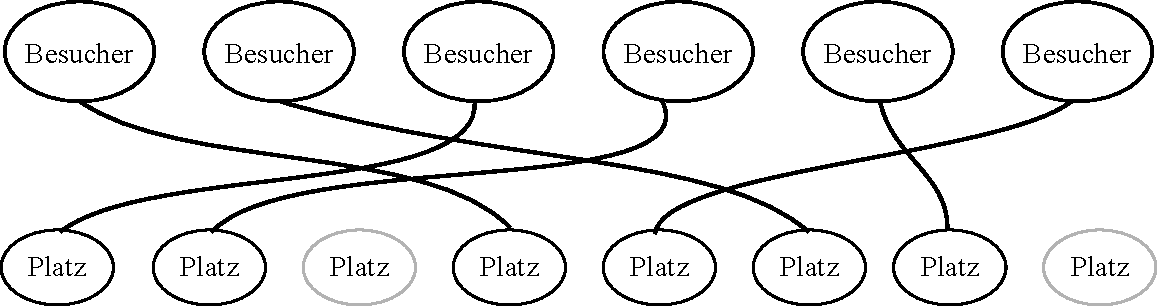
\includegraphics[scale=0.5]{Kinoabbildungen.pdf}
	\end{figure}
\end{frame}

%\begin{frame}
%	\frametitle{Lösung}
%	\textit{In dieser Teilaufgabe nehmen wir an, 6 Kinobesucher besuchten ein Kino mit 8 Plätzen. Wie viele injektive Abbildungen gibt es?} \\[2em] \pause
%	
%	Es gibt insgesamt $$8 \cdot 7 \cdot 6 \cdot 5 \cdot 4 \cdot 3 = 20160$$ injektive Abbildungen. \\[1em]
%	Der erste Besucher hat 8 Plätze zur Auswahl. Da aufgrund der Injektivität der nächste Besucher einen anderen Sitzplatz wählen muss, stehen ihm noch 7 Plätze zur Auswahl. Dies kann man für die restlichen Besucher fortsetzen.
%	
%\end{frame}

\subsection{Aufgabe 2}
\begin{frame}{Aufgabe 2}
	
	Was kann man über die Surjektivität, Injektivität und Bijektivität folgender Abbildungen sagen? Begründet jeweils kurz.
	\visible<+(-1)>{}
	\begin{alist}
		\item $f \from \R \functionto \R, \; x \mapsto x^2$ \\
		\visible<+-|handout:2->{
			Weder injektiv ($f(-2) = f(2) = 4$) noch surjektiv (auf $-1 \in \R$ wird nicht abgebildet) \impl auch nicht bijektiv.
		}
		\item $f \from \R_+ \functionto \R_+, \; x \mapsto x^2$ \\
		\visible<+-|handout:2->{
			Wir können zu jedem $y \in \R_+$ ein $x \in \R_+$ angeben, so dass $f(x) = y$, nämlich $ x = \sqrt{y}$. \\
			\impl surjektiv, und da dieses $x$ eindeutig ist auch injektiv \impl bijektiv.
		}
		
		\item $f \from \N_0 \functionto \N_0, \; x \mapsto \casesl{ 42 & \text{wenn $x = 0$} \\ x - 1 & \text{sonst} }$ \\
		\visible<+-|handout:2->{
			Nicht injektiv ($f(0) = f(43) = 42$), aber surjektiv (Für jedes $x \in \N_0$ gilt: $x + 1 \in \N_0 \text{ und } f(x+1) = x$) \\ \impl nicht bijektiv.
		} 
	\end{alist}
\end{frame}



\begin{frame}[t]
	\begin{block}{Wahr oder Falsch?}
		Sei $M$ eine beliebige endliche Menge und $f$ eine Abbildung $f \from M \functionto M$. \\
			\TrueQuestion{Wenn $f$ injektiv ist, dann ist $f$ auch surjektiv.}
			\TrueQuestion{Wenn $f$ surjektiv ist, dann ist $f$ auch injektiv}
			\FalseQuestionE{Die beiden Aussagen gelten auch, wenn $M$ nicht endlich ist.}{Gegenbeispiele: \\ 
				$f \from \N_0 \functionto \N_0, n \mapsto 2 \· n $ \\ 
				$g \from \N_0 \functionto \N_0, n \mapsto \floor{\dfract n/2 }$}
	\end{block}
	
\end{frame}

\section{Wörter}

\begin{frame}
	\frametitle{Wörter}
	\begin{block}{Definition}
		\begin{itemize}
			\item Ein \textbf{Alphabet} ist eine endliche Menge von Zeichen. \pause
			\item Ein \textbf{Wort} $w$  über einem Alphabet A ist ein \textbf{endliche Folge von Zeichen} aus A \\ \pause
				\emph{Formal}: Eine surjektive Abbildung $f : \nZ_n \to A$\\[0.5em]
				Zur Erinnerung: $ \nZ_n = \{i\in \nN_0 \mid 0 \leq i < n \} $ 
		\end{itemize}
	\end{block}	

	\pause
	\begin{block}{Definition}
		Ist $A$ ein Alphabet, dann ist $A^*$ die \textbf{Menge aller Wörter}, die nur Zeichen aus $A$ enthalten, also:\\
		\pause 
		$A^*$ ist die Menge aller Abbildungen $w: \nZ_n \to B$ mit $n \in \nN_0$ und $B \subseteq A$. \\
	\end{block}

	\pause
	\begin{block}{Beispiel}
		Sei $ A = \{ a,b\} $ ein Alphabet. 
		Dann sind $ w_1 = aabbabab$ und $w_2 = ab $ zwei mögliche Wörter.
		Es gilt also $ w_1 \in A^*, w_2 \in A^*$
	\end{block}

\end{frame}

\begin{frame}
	\frametitle{Das Leere Wort}
	\begin{block}{Definition}
		Wir definieren das \textbf{leere Wort} als $$ \varepsilon := \nZ_0  \to A \qquad \varepsilon := \{\} \to \{\}$$ \pause
		Es gilt $ \varepsilon \circ w \circ \varepsilon = w \;$ (Beweis: VL) \\[1em] \pause
		
		Wichtig: Das leere Wort ist auch ein \enquote{echtes, gleichberechtigtes} Wort. Die Null ist bei den natürlichen Zahlen ja auch nicht einfach \enquote{nichts}. \\[1em] \pause
		
		Ist $\varepsilon := \{\} \to \{\}$ eine Relation? Und eine Funktion? Ist es surjektiv? \\ \pause
		Bemerkung: In der formalen Definition fordern wir die Surjektivität der Funktion, damit das leere Wort eindeutig ist!
	\end{block}
	
\end{frame}


\begin{frame}
	\frametitle{Konkatenation}
	\begin{block}{}
		Sei $w_1 = $ Schrank , $w_2 = $ Schlüssel \\
		Dann gilt $ w_1 \circ w_2 = \text{SchrankSchlüssel} \neq w_2 \circ w_1 = \text{SchlüsselSchrank}$\\ \pause
		Konkatenation ist also \textbf{nicht kommutativ!} \\
		Ist sie \textbf{assoziativ}? \pause Ja!		
	\end{block}

	\begin{block}{Beobachtung}
		Falls $w=w_1\circ w_2 $ und $w_1 \in A^* , w_2 \in B^* $, dann gilt
		$ w\in (A\cup B)^* $ 
	\end{block}

	\begin{block}{Mehrfachkonkatenation}
		\begin{align*}
			w^0 &= \varepsilon \\
			w^k &= \underbrace{w\circ w\circ \cdots \circ w}_{k-mal}
		\end{align*}

	\end{block}

\end{frame}

\begin{frame}
	\frametitle{Länge von Wörtern}
	\begin{block}{Definition}
		Unter der \textbf{Länge} eines Wortes versteht man die Anzahl der Zeichen, aus der das Wort besteht.
	\end{block}

	
	\begin{block}{Beispiel}
		$ \vert \text{hallo} \vert = \pause 5 $ \\
		$ \vert \varepsilon \vert = \pause 0 $
	\end{block}

	\pause
	\begin{block}{Lemma}
		$$ \vert a\circ b \vert = \vert a \vert + \vert b \vert $$
	\end{block}

	\pause
	\begin{block}{Lemma}
		$$ \vert w^k \vert = k \vert w \vert $$
	\end{block}
\end{frame}

\begin{frame}
	\frametitle{Wörter}
	$A^n$: \emph{Menge aller Wörter der Länge $n$} über dem Alphabet $A$.\\
	Wie kann man damit $A^*$ ausdrücken? \\
	\pause
	\[ A^\ast = \bigcup \limits_{i = 0}^\infty A^i \]
	
	\pause
	\begin{block}{Rückblick}
		\begin{align*}
		\bigcup_{i\in I} M_i &= \{ x \mid \text{es gibt ein } i\in I \text{ so, dass } x\in  M_i \}  \;
		\end{align*}
	\end{block}
\end{frame}

\begin{frame}
	\frametitle{Aufgabe}
	\begin{itemize}
		\item Welche Wörter lassen sich aus dem Alphabet $A = \{a , b \}$ bilden? Was enthält die Menge $A^*$?
		\item Ist das Wort $w =$ \code{aabb}$\,\cdot\,$\code{ba} ein Element der Menge $A^5$?
		\item Was ist $A^2 \times A^2$? \\
			Wir definieren die Abbildung $f : A^* \times A^* \to A^*, \; (w_1, w_2) \mapsto w_1 \cdot w_2$ \\
			Was ist $f(A^2 \times A^2)$?
	\end{itemize}
\end{frame}

\begin{frame}
	\frametitle{Lösung}
	\textit{Welche Wörter lassen sich aus dem Alphabet $A = \{a , b \}$ bilden? Was enthält die Menge $A^*$?} \\[2em] \pause
	
	Aus $A$ lassen sich z.B. die Wörter $$\text{a, b, aa, bb, ab, ba, aaa, bbb, }\dots$$ bilden. Die Menge $A^*$ enthält gerade diese Wörter.\\
	\pause
	Beachte: Auch $\varepsilon$ ist in $A^*$!
\end{frame}

\begin{frame}
	\frametitle{Lösung}
	\textit{Ist das Wort $w =$ \code{aabb}$\,\cdot\,$\code{ba} ein Element der Menge $A^5$?} \\[2em] \pause
	
	Nein. Es gilt $w = \textbf{aabbba}$. Das Wort besteht zwar aus Symbolen, die alle in $A$ liegen, ist aber 6 Zeichen lang.
\end{frame}

\begin{frame}
	\frametitle{Lösung}
	\textit{Was ist $A^2 \times A^2$? \\
		Wir definieren die Abbildung $f : A^* \times A^* \to A^*, \; (w_1, w_2) \mapsto w_1 \cdot w_2$ \\
		Was ist $f(A^2 \times A^2)$?} \\[2em]  \pause
	
	 $$ A^2 \times A^2 = \{\mathbf{(aa,aa),(aa,bb),(aa,ab),(aa,ba),(bb,aa),} \dots \}$$
	 \pause
	 $$ f(A^2 \times A^2) = \{\mathbf{aaaa, aabb, aaab, aaba, bbaa,} \dots \} = A^4 $$
\end{frame}

\begin{frame}	
	\begin{block}{Was ihr nun wissen solltet}
		\begin{itemize}
			\item Wie man mit Relationen umgeht
			\item Welche Eigenschaften Relationen haben können
			\item Was Abbildungen sind und welche Eigenschaften sie haben können
			\item Wie man mit Wörtern rechnet
		\end{itemize}
	\end{block}
	
	\begin{block}{Was nächstes Mal kommt}
		\begin{itemize}
			\item Sinnvollere Gebilde als \word{retsinnaL\sp nosrO} mit \emph{formalen Sprachen}
			\item Endlich mal logische Aussagen mit \emph{Aussagenlogik}
		\end{itemize}
	\end{block}
\end{frame}

%% Letzte Seite
\lastframe{0.68}{0}{xkcd/identity.png}{http://www.xkcd.com/1121/}

\slideThanks

\end{document}